\section{The team's allocation of time and resources}
\label{sec:timeSpent}
This section presents an overview of actual time spent and an evaluation of the allocation of resources.

\subsection{Time spent}
At the beginning of the project, the team made an estimation on how much time that would be spent on each section of the project. This is shown in table~\ref{tab:timeEstWP}. The actual distribution is shown in figure~\ref{fig:piechart}.

\begin{figure}[H]
\centering
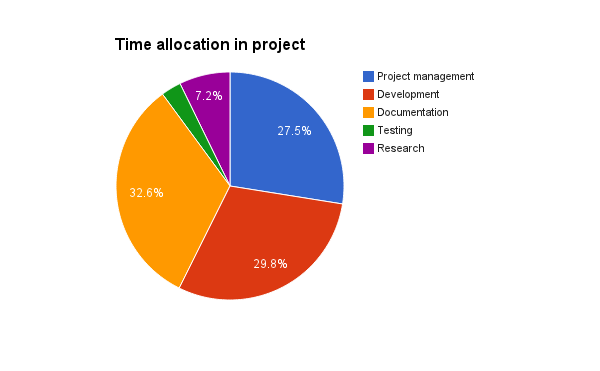
\includegraphics[width=0.6\textwidth, clip, trim=4cm 2cm 4cm 1cm]{ch/retrospect/fig/timePie.png}
\caption{Pie chart of time spent on different parts of the project}
\label{fig:piechart}
\end{figure}

\begin{figure}[H]
\centering
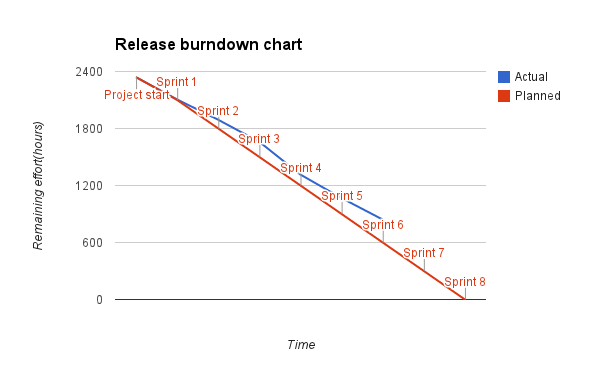
\includegraphics[width=0.7\textwidth, clip, trim=1.1cm 0.5cm 1.2cm 1cm]{ch/retrospect/fig/release.png}
\caption{Project release burn down chart}
\label{fig:release}
\end{figure}

When comparing the actual time spent to the estimated time, it is clear that the team's initial estimations does not match the actual time spent. This is illustrated in~\ref{fig:release}.

There are several reasons for this, including unplanned absence of team members, underestimation of tasks and too heavy workload due to deliveries in other classes. The subsequent sections will elaborate on some of these deviations.

\subsubsection{Deviations in testing}
One of the larger deviations is the time devoted to testing. The time logged for testing is more than three times lower than the 10\% that was estimated. This is because the time logged for testing only was time that was spent exclusively on testing, mainly including user testing. The acceptance testing with the customer was performed during the customer meetings and is therefore logged as project management. Much of the time spent on running functional tests was also logged as development instead of testing. With this in mind, the actual time spent on testing is closer to the estimated amount.

\subsubsection{Deviations in project management}
The largest abnormality lies in the project management, logging a total of 27.5\% of the spent time, which is five times more than the original estimate. 

There are several factors for this, the most influencial factor being poor estimation done in an early stage of the project. This was due to lack of experience. 

The project management consists mainly of hours logged for meetings. Many of the meetings had agendas that could classify them as either development or research. For example, the early prototyping of the user interface was done during prolonged meetings, and was logged as project management. 

In retrospect, the project management should have been specified differently, or the meetings should have been dedicated to development or research, and time spent should be logged accordingly.

\subsection{Resource allocation}
As described in section~\ref{sec:availResources}, the team had several resources available, including a supervisor, and the customer. The team had internal meetings at least two times a week, and also an eight hour work session once a week. In addition, weekly meetings with the customer and meetings with the supervisor every other week were held.

To have meetings on such a regular basis has been of great value. It saved a lot of time to have pre-booked meeting rooms, and it was easier for the parties involved in the project to prepare for the meetings.
\subsubsection{Externally}
During the meetings with the supervisor, the team were given valuable input and feedback regarding customer relations, and the content and structure of the report. The role of the supervisor was unclear to the team in the early stages of the project. It was quickly learned that he was more to guide us rather than supervise us. The only real oversight the supervisor had was the activity report which included a work log and a summary of the progress made since the last meeting.

Communicating with the customer on a regular basis reduced the probability of misunderstandings to arise and increased the likelihood that the team would deliver a product the customer would be greatly satisfied with.
 
\subsubsection{Internally}
One of the most valuable decisions that was made in this project was to actually have fixed meeting times. This assured that the entire team was kept updated and involved. On these internal meetings, the team planned and distributed tasks among the team members, and discussed occurring issues. Each team member was assigned an area of responsibility, so that no important parts of the project would be neglected. It also turned out to be a way to keep the motivation high and further involve the team members.


The largest factor in the deviation, however, was the change from 20 to 25 work hours per week as described in section~\ref{sec:availableHours}. Had the team not travelled to China, the project would have had 9 sprints worth a total of 2160 hours to spend on the project. The team's attempt to compensate for the school trip left the team with 8 sprints, giving a total of 2340 working hours, as shown in table~\ref{tab:availHours}. This means that the team projected a usage of 180 hours more than the course required.

